% Arquivo LaTeX de exemplo de dissertação/tese a ser apresentada à CPG do IME-USP
%
% Criação: Jesús P. Mena-Chalco
% Revisão: Fabio Kon e Paulo Feofiloff
% Adaptação para UTF8, biblatex e outras melhorias: Nelson Lago
%
% Except where otherwise indicated, these files are distributed under
% the MIT Licence. The example text, which includes the tutorial and
% examples as well as the explanatory comments in the source, are
% available under the Creative Commons Attribution International
% Licence, v4.0 (CC-BY 4.0) - https://creativecommons.org/licenses/by/4.0/


%%%%%%%%%%%%%%%%%%%%%%%%%%%%%%%%%%%%%%%%%%%%%%%%%%%%%%%%%%%%%%%%%%%%%%%%%%%%%%%%
%%%%%%%%%%%%%%%%%%%%%%%%%%%%%%% PREÂMBULO LaTeX %%%%%%%%%%%%%%%%%%%%%%%%%%%%%%%%
%%%%%%%%%%%%%%%%%%%%%%%%%%%%%%%%%%%%%%%%%%%%%%%%%%%%%%%%%%%%%%%%%%%%%%%%%%%%%%%%

% A opção twoside (frente-e-verso) significa que a aparência das páginas pares
% e ímpares pode ser diferente. Por exemplo, as margens podem ser diferentes ou
% os números de página podem aparecer à direita ou à esquerda alternadamente.
% Mas nada impede que você crie um documento "só frente" e, ao imprimir, faça
% a impressão frente-e-verso.
%
% Aqui também definimos a língua padrão do documento (a última da lista) e
% línguas adicionais. Para teses do IME, no mínimo português e inglês são
% obrigatórios, porque independentemente da língua principal do texto é
% preciso fornecer o resumo nessas duas línguas. LaTeX aceita alguns nomes
% diferentes para a língua portuguesa; dentre as opções, prefira sempre
% "brazilian" para português brasileiro e "portuguese" para português europeu.
%\documentclass[a4paper,12pt,twoside,brazilian,english]{book}
\documentclass[a4paper,12pt,twoside,english,brazilian]{book}

% O preâmbulo de um documento LaTeX pode ser razoavelmente longo. Neste
% modelo, optamos por reduzi-lo, colocando praticamente tudo do preâmbulo
% nas packages "imegoodies" e "imelooks".
%
% imegoodies carrega diversas packages muito úteis e populares (algumas
% são praticamente obrigatórias, como amsmath, babel, array etc.). É
% uma boa ideia usá-la com outros documentos também. Ela inclui vários
% comentários explicativos e dicas de uso; não tenha medo de alterá-la
% conforme a necessidade.
%
% imelooks carrega algumas packages e configurações que definem a
% aparência do documento; você também pode querer usá-la (ou partes
% dela) com outros documentos para obter as mesmas fontes, margens
% etc. Tal como "imegoodies", pode valer a pena ler os comentários
% e fazer modificações nessa package. Com a opção "thesis", imelooks
% também define os comandos para capa, folha de rosto etc.
\usepackage{imegoodies}
\usepackage[thesis]{imelooks}

%\nocolorlinks % para impressão em P&B

% Diretórios onde estão as figuras; com isso, não é necessário (mas
% é permitido) colocar o caminho completo em \includegraphics. Note
% que a extensão nunca é necessária (mas é permitida), ou seja, o
% resultado é o mesmo com "\includegraphics{figuras/foto.jpeg}",
% "\includegraphics{foto.jpeg}", "\includegraphics{figuras/foto}"
% ou "\includegraphics{foto}".
\graphicspath{{figuras/},{fig/},{logos/},{img/},{images/},{imagens/}}

% Comandos rápidos para mudar de língua:
% \en -> muda para o inglês
% \br -> muda para o português
% \texten{blah} -> o texto "blah" é em inglês
% \textbr{blah} -> o texto "blah" é em português
\babeltags{br = brazilian, en = english}


%%%%%%%%%%%%%%%%%%%%%%%%%%%%%%%%%%%%%%%%%%%%%%%%%%%%%%%%%%%%%%%%%%%%%%%%%%%%%%%%
%%%%%%%%%%%%%%%%%%%%%%%%%%%%%%%%%% METADADOS %%%%%%%%%%%%%%%%%%%%%%%%%%%%%%%%%%%
%%%%%%%%%%%%%%%%%%%%%%%%%%%%%%%%%%%%%%%%%%%%%%%%%%%%%%%%%%%%%%%%%%%%%%%%%%%%%%%%

% O arquivo com os dados bibliográficos para biblatex; você pode usar
% este comando mais de uma vez para acrescentar múltiplos arquivos
\addbibresource{bibliografia.bib}

% Este comando permite acrescentar itens à lista de referências sem incluir
% uma referência de fato no texto (pode ser usado em qualquer lugar do texto)
%\nocite{bronevetsky02,schmidt03:MSc, FSF:GNU-GPL, CORBA:spec, MenaChalco08}
% Com este comando, todos os itens do arquivo .bib são incluídos na lista
% de referências
%\nocite{*}

% É possível definir como determinadas palavras podem (ou não) ser
% hifenizadas; no entanto, a hifenização automática geralmente funciona bem
\babelhyphenation{documentclass latexmk soft-ware clsguide} % todas as línguas
\babelhyphenation[brazilian]{Fu-la-no}
\babelhyphenation[english]{what-ever}

% Estes comandos definem o título e autoria do trabalho e devem sempre ser
% definidos, pois além de serem utilizados para criar a capa, também são
% armazenados nos metadados do PDF. O subtítulo é opcional.
\title{Modelo de Lorenz 80: Uma abordagem estocástica }
\translatedtitle{The Lorenz 80 model: a stochastic approach}

\author{Lucas Amaral Taylor}

\def\profa{Prof\kern.02em.\kern-.07emª\kern.07em}
\def\dra{Dr\kern-.04em.\kern-.11emª\kern.07em}

% Para TCCs, este comando define o supervisor
\orientador{Prof. Dr. Breno Raphaldini Ferreira da Silva}


\banca{
  \profa{} \dra{} Fulana de Tal (orientadora) -- IME-USP [sem ponto final],
  % Em inglês, não há o "ª"
  %Prof. Dr. Fulana de Tal (advisor) -- IME-USP [sem ponto final],
  Prof. Dr. Ciclano de Tal -- IME-USP [sem ponto final],
  \profa{} \dra{} Convidada de Tal -- IMPA [sem ponto final],
}

% A página de rosto da versão para depósito (ou seja, a versão final
% antes da defesa) deve ser diferente da página de rosto da versão
% definitiva (ou seja, a versão final após a incorporação das sugestões
% da banca).
\tipotese{
  %mestrado,
  %doutorado,
  tcc,
  %definitiva, % É a versão para defesa ou a versão definitiva?
  %quali, % É qualificação?
  programa={Matemática Aplicada e Computacional},
}

\defesa{
  local={São Paulo},
  data=2025-11-01, % YYYY-MM-DD
}

% Se não houve bolsa, remova
%
% Norma sobre agradecimento por auxílios da FAPESP:
% https://fapesp.br/11789/referencia-ao-apoio-da-fapesp-em-todas-as-formas-de-divulgacao
%
% Norma sobre agradecimento por auxílios da CAPES (Portaria 206,
% de 4 de Setembro de 2018):
% https://www.in.gov.br/materia/-/asset_publisher/Kujrw0TZC2Mb/content/id/39729251/do1-2018-09-05-portaria-n-206-de-4-de-setembro-de-2018-39729135
%
%\apoio{O presente trabalho foi realizado com apoio da Coordenação
%      de Aperfeiçoamento\\ de Pessoal de Nível Superior -- Brasil
%      (CAPES) -- Código de Financiamento 001} % o código é sempre 001
%
%\apoio{This study was financed in part by the Coordenação de
%      Aperfeiçoamento\\ de Pessoal de Nível Superior -- Brasil
%      (CAPES) -- Finance Code 001} % o código é sempre 001
%
%\apoio{Durante o desenvolvimento deste trabalho, o autor recebeu\\
%      auxílio financeiro da FAPESP -- processo nº aaaa/nnnnn-d}
%
%\apoio{During the development if this work, the author received\\
%      financial support from FAPESP -- grant \#aaaa/nnnnn-d}
\apoio{}

% A licença do seu trabalho. Use CC-BY, CC-BY-NC, CC-BY-ND, CC-BY-SA,
% CC-BY-NC-SA ou CC-BY-NC-ND para escolher a licença Creative Commons
% correspondente (o sistema insere automaticamente o texto da licença).
% Se quiser estabelecer regras diferentes para o uso de seu trabalho,
% converse com seu orientador e coloque o texto da licença aqui, mas
% observe que apenas TCCs sob alguma licença Creative Commons serão
% acrescentados ao BDTA. Se você tem alguma intenção de publicar o
% trabalho comercialmente no futuro, sugerimos a licença CC-BY-NC-ND.
%
%\direitos{CC-BY-NC-ND}
%
%\direitos{Autorizo a reprodução e divulgação total ou parcial deste
%          trabalho, por qualquer meio convencional ou eletrônico,
%          para fins de estudo e pesquisa, desde que citada a fonte.}
%
%\direitos{I authorize the complete or partial reproduction and disclosure
%          of this work by any conventional or electronic means for study
%          and research purposes, provided that the source is acknowledged.}
%
\direitos{CC-BY}

% Para gerar a ficha catalográfica, acesse https://fc.ime.usp.br/,
% preencha o formulário e escolha a opção "Gerar Código LaTeX".
% Basta copiar e colar o resultado aqui.
\fichacatalografica{}


%%%%%%%%%%%%%%%%%%%%%%%%%%%%%%%%%%%%%%%%%%%%%%%%%%%%%%%%%%%%%%%%%%%%%%%%%%%%%%%%
%%%%%%%%%%%%%%%%%%%%%%% AQUI COMEÇA O CONTEÚDO DE FATO %%%%%%%%%%%%%%%%%%%%%%%%%
%%%%%%%%%%%%%%%%%%%%%%%%%%%%%%%%%%%%%%%%%%%%%%%%%%%%%%%%%%%%%%%%%%%%%%%%%%%%%%%%

\begin{document}

%%%%%%%%%%%%%%%%%%%%%%%%%%% CAPA E PÁGINAS INICIAIS %%%%%%%%%%%%%%%%%%%%%%%%%%%%

% Aqui começa o conteúdo inicial que aparece antes do capítulo 1, ou seja,
% página de rosto, resumo, sumário etc. O comando frontmatter faz números
% de página aparecem em algarismos romanos ao invés de arábicos e
% desabilita a contagem de capítulos.
\frontmatter

\pagestyle{plain}

\onehalfspacing % Espaçamento 1,5 na capa e páginas iniciais

\maketitle % capa e folha de rosto

%%%%%%%%%%%%%%%% DEDICATÓRIA, AGRADECIMENTOS, RESUMO/ABSTRACT %%%%%%%%%%%%%%%%%%

\begin{dedicatoria}
Na verdade, na verdade vos digo que, se o grão de trigo, caindo na terra, não morrer, fica ele só; mas se morrer, dá muito fruto. 

João 12:24
\end{dedicatoria}

% Reinicia o contador de páginas (a próxima página recebe o número "i") para
% que a página da dedicatória não seja contada.
\pagenumbering{roman}

% Agradecimentos:
% Se o candidato não quer fazer agradecimentos, deve simplesmente eliminar
% esta página. A epígrafe, obviamente, é opcional; é possível colocar
% epígrafes em todos os capítulos. O comando "\chapter*" faz esta seção
% não ser incluída no sumário.
\chapter*{Agradecimentos}
\epigrafe{Do. Or do not. There is no try.}{Mestre Yoda}

Texto texto texto texto texto texto texto texto texto texto texto texto texto
texto texto texto texto texto texto texto texto texto texto texto texto texto
texto texto texto texto texto texto texto texto texto texto texto texto texto
texto texto texto texto. Texto opcional.

%!TeX root=../tese.tex
%("dica" para o editor de texto: este arquivo é parte de um documento maior)
% para saber mais: https://tex.stackexchange.com/q/78101

% As palavras-chave são obrigatórias, em português e em inglês, e devem ser
% definidas antes do resumo/abstract. Acrescente quantas forem necessárias.
\palavraschave{Palavra-chave1, Palavra-chave2, Palavra-chave3}

\keywords{Keyword1,Keyword2,Keyword3}

% O resumo é obrigatório, em português e inglês. Estes comandos também
% geram automaticamente a referência para o próprio documento, conforme
% as normas sugeridas da USP.
\resumo{
Elemento obrigatório, constituído de uma sequência de frases concisas e
objetivas, em forma de texto. Deve apresentar os objetivos, métodos empregados,
resultados e conclusões. O resumo deve ser redigido em parágrafo único, conter
no máximo 500 palavras e ser seguido dos termos representativos do conteúdo do
trabalho (palavras-chave). Deve ser precedido da referência do documento.
Texto texto texto texto texto texto texto texto texto texto texto texto texto
texto texto texto texto texto texto texto texto texto texto texto texto texto
texto texto texto texto texto texto texto texto texto texto texto texto texto
texto texto texto texto texto texto texto texto texto texto texto texto texto
texto texto texto texto texto texto texto texto texto texto texto texto texto
texto texto texto texto texto texto texto texto.
Texto texto texto texto texto texto texto texto texto texto texto texto texto
texto texto texto texto texto texto texto texto texto texto texto texto texto
texto texto texto texto texto texto texto texto texto texto texto texto texto
texto texto texto texto texto texto texto texto texto texto texto texto texto
texto texto.
}

\abstract{
Elemento obrigatório, elaborado com as mesmas características do resumo em
língua portuguesa. De acordo com o Regimento da Pós-Graduação da USP (Artigo
99), deve ser redigido em inglês para fins de divulgação. É uma boa ideia usar
o sítio \url{www.grammarly.com} na preparação de textos em inglês.
Text text text text text text text text text text text text text text text text
text text text text text text text text text text text text text text text text
text text text text text text text text text text text text text text text text
text text text text text text text text text text text text.
Text text text text text text text text text text text text text text text text
text text text text text text text text text text text text text text text text
text text text.
}



%%%%%%%%%%%%%%%%%%%%%%%%%%% LISTAS DE FIGURAS ETC. %%%%%%%%%%%%%%%%%%%%%%%%%%%%%

% Como as listas que se seguem podem não incluir uma quebra de página
% obrigatória, inserimos uma quebra manualmente aqui.
\cleardoublepage

% Todas as listas são opcionais; Usando "\chapter*" elas não são incluídas
% no sumário. As listas geradas automaticamente também não são incluídas por
% conta das opções "notlot" e "notlof" que usamos para a package tocbibind.

% Normalmente, "\chapter*" faz o novo capítulo iniciar em uma nova página, e as
% listas geradas automaticamente também por padrão ficam em páginas separadas.
% Como cada uma destas listas é muito curta, não faz muito sentido fazer isso
% aqui, então usamos este comando para desabilitar essas quebras de página.
% Se você preferir, comente as linhas com esse comando e des-comente as linhas
% sem ele para criar as listas em páginas separadas. Observe que você também
% pode inserir quebras de página manualmente (com \clearpage, veja o exemplo
% mais abaixo).
\newcommand\disablenewpage[1]{{\let\clearpage\par\let\cleardoublepage\par #1}}

% Nestas listas, é melhor usar "raggedbottom" (veja basics.tex). Colocamos
% a opção correspondente e as listas dentro de um grupo para ativar
% raggedbottom apenas temporariamente.
\bgroup
\raggedbottom

% Quebra de página manual
\clearpage

%%%%% Listas criadas automaticamente

% Você pode escolher se quer ou não permitir a quebra de página
%\listoffigures
\disablenewpage{\listoffigures}

% Você pode escolher se quer ou não permitir a quebra de página
%\listoftables
\disablenewpage{\listoftables}

% Esta lista é criada "automaticamente" pela package float quando
% definimos o novo tipo de float "program" (em utils.tex)
% Você pode escolher se quer ou não permitir a quebra de página
%\listof{program}{\programlistname}
\disablenewpage{\listof{program}{\programlistname}}

% Sumário (obrigatório)
\tableofcontents

\egroup % Final de "raggedbottom"

% Referências indiretas ("x", veja "y") para o índice remissivo (opcionais,
% pois o índice é opcional). É comum colocar esses itens no final do documento,
% junto com o comando \printindex, mas em alguns casos isso torna necessário
% executar texindy (ou makeindex) mais de uma vez, então colocar aqui é melhor.
\index{Inglês|see{Língua estrangeira}}
\index{Figuras|see{Floats}}
\index{Tabelas|see{Floats}}
\index{Código-fonte|see{Floats}}
\index{Subcaptions|see{Subfiguras}}
\index{Sublegendas|see{Subfiguras}}
\index{Equações|see{Modo matemático}}
\index{Fórmulas|see{Modo matemático}}
\index{Rodapé, notas|see{Notas de rodapé}}
\index{Captions|see{Legendas}}
\index{Versão original|see{Tese/Dissertação, versões}}
\index{Versão corrigida|see{Tese/Dissertação, versões}}
\index{Palavras estrangeiras|see{Língua estrangeira}}
\index{Floats!Algoritmo|see{Floats, ordem}}


%%%%%%%%%%%%%%%%%%%%%%%%%%%%%%%% CAPÍTULOS %%%%%%%%%%%%%%%%%%%%%%%%%%%%%%%%%%%%%

% Aqui vai o conteúdo principal do trabalho, ou seja, os capítulos que compõem
% a dissertação/tese. O comando mainmatter reinicia a contagem de páginas,
% modifica a numeração para números arábicos e ativa a contagem de capítulos.
\mainmatter

\pagestyle{mainmatter}

% Espaçamento simples
\singlespacing

% A introdução não tem número de capítulo, então os cabeçalhos também não
\pagestyle{unnumberedchapter}
%!TeX root=../tese.tex
%("dica" para o editor de texto: este arquivo é parte de um documento maior)
% para saber mais: https://tex.stackexchange.com/q/78101

%% ------------------------------------------------------------------------- %%

% "\chapter" cria um capítulo com número e o coloca no sumário; "\chapter*"
% cria um capítulo sem número e não o coloca no sumário. A introdução não
% deve ser numerada, mas deve aparecer no sumário. Por conta disso, este
% modelo define o comando "\chapter**".
\chapter**{Introdução}
\label{cap:introducao}

\enlargethispage{.5\baselineskip}
Lorem
\pagestyle{mainmatter}
\chapter{O modelo de Lorenz 80 determinístico} \label{cap:ch01_lorenz_deterministico}

\section{Introdução} \label{sec:ch01_introducao}
Este capítulo tem como objetivo apresentar o modelo determinístico Lorenz 80. Para isso, começamos, na seção \ref{sec:ch01_geofisica}, com uma introdução aos conceitos básicos de geofísica, a fim de familiarizar o leitor com os fundamentos dessa área. Em seguida, na seção \ref{sec:ch01_apresentacao_do_modelo}, contextualizamos o modelo, discutindo os trabalhos que o precederam e as motivações por trás de sua formulação.

Na seção \ref{sec:ch01_agua_rasa}, introduzimos o modelo de água rasa, que serve de base para o desenvolvimento do Lorenz 80. A construção deste é detalhada na seção \ref{sec:ch01_construcao_do_modelo}. Por fim, a seção \ref{sec:ch01_simulacoes_deterministico} traz simulações computacionais realizadas com o modelo, acompanhadas de uma análise gráfica dos resultados.

\section{Breves considerações sobre geofísica} \label{sec:ch01_geofisica}

Nesta seção, reunimos um breve glossário com os principais conceitos de geofísica que servem de base para a compreensão do modelo de Lorenz 80. Todas as definições expostas abaixo estão detalhadas em \citet{Vallis2017}.
\begin{itemize}
    \item \textbf{Convecção.} Convecção é um processo de transferência de calor que ocorre em
    fluidos, como líquidos e gases. Esse fenômeno envolve o movimento do próprio
    fluido e a transferência energia térmica de uma região para outra.
	\item \textbf{Parâmetro de Coriolis.} A \textit{força de Coriolis} é uma quasi-força (ou pseudo-força) que surge devido à rotação da Terra. Quando analisamos o movimento de um corpo em um referencial rotativo, esse corpo parece sofrer a ação de uma força que desvia sua trajetória. Esse desvio é quantificado pelo parâmetro de Coriolis, definido pela expressão:
	      \begin{equation*}
	      	f = 2 \Omega \sin(\theta)
	      \end{equation*}
	      onde $\Omega$ representa a velocidade angular de rotação da Terra e $\theta$ é a latitude, ou seja, o ângulo entre a posição do ponto e o equador terrestre.
	      
	\item \textbf{Número de Rossby.} O número de Rossby é a razão entre a magnitude da aceleração relativa e a aceleração de Coriolis. É aproximado por:
	      \begin{equation*}
	      	Ro \equiv \frac{U}{fL},
	      \end{equation*}
	      
	      onde $U$ é a magnitude aproximada da velocidade horizontal e $L$ é uma escala de comprimento e $f$ é o parâmetro de Coriolis.
	      
	\item \textbf{Equilíbrio hidrostático.} Matematicamente, a equação do equilíbrio hidrostático é dada por:
	      \begin{equation}
	      	\frac{\partial p}{\partial z} = - \rho_0g, \label{eq:equilibrio_hidrostatico}
	      \end{equation}
	          
	      onde: $p$ é a pressão do fluido, $z$ é a coordenada vertical, $\rho_0$ é a densidade constante do fluido e $g$ é a aceleração da gravidade.
	\item \textbf{Conservação de massa.} Em um escoamento de fluido, a densidade pode variar de acordo com o tempo ou a posição. No entanto, a \textit{quantidade total de massa} do fluido permanece constante. Esse princípio estabelece que a massa não pode ser criada nem perdida durante o movimento.
	      
	\item \textbf{Equações quasi-geostróficas.} As equações quasi-geostróficas são equações  amplamente usadas em estudos teóricos da atmosfera e oceano. Elas atendem as seguintes características:
	      \begin{enumerate}
	      	\item O número de Rossby é pequeno;
	      	\item A escala do movimento não é significativamente maior do que a escala de deformação;
	      	\item As variações no parâmetro de Coriolis são pequenas;
	      	\item As escalas de tempo são advectivas, ou seja, $T=L/U$.
	      \end{enumerate}
\end{itemize}



\section{Motivação e apresentação do modelo} \label{sec:ch01_apresentacao_do_modelo}

Edward Norton Lorenz (1917-2008) foi um importante matemático e meteorologista responsável pela publicação de vários artigos com desenvolvimento de modelos na área de meteorologia e geofísica.

O mais famoso deles foi o artigo \textit{``Deterministic Nonperiodic Flow''}, publicado em 1963 \citet{Lorenz1963}. Nele, Lorenz desenvolveu um modelo matemático simplificado para a convecção atmosférica, composto por três equações diferenciais ordinárias, expressas abaixo:
\begin{align}
    \begin{cases}
        \frac{dx}{dt} & = \sigma(y-x)     \\
        \frac{dy}{dt} & = x(\rho - z) - y \\
        \frac{dz}{dt} & = xy - \beta z
    \end{cases},
    \label{eq:ch01-lorenz63}
\end{align}

onde $\sigma$ é o \textit{número de Prandtl}, que regula a sensibilidade entre $x$ e $y$; $\rho$ é o \textit{número de Rayleigh}, associado à magnitude da convecção; e $\beta$ está ligado à geometria da célula de convecção, influenciando a relação entre as taxas de $x$ e $z$.
    
O modelo acima, conhecido como Lorenz 63, é um sistema determinístico desenvolvido para representar sistemas hidrodinâmicos ideais e dissipativos de força. O Lorenz 63 tornou-se amplamente conhecido por sua alta sensibilidade às condições iniciais — pequenas alterações nas variáveis $x_0$, $y_0$ e $z_0$ podem levar a trajetórias completamente distintas no espaço de fases. Essa sensibilidade extrema é uma característica caótica do modelo.

Em 1980, Lorenz publica o artigo intitulado ``\textit{Attractor Sets and Quasi-Geostrophic Equilibrium }'' \citep{Lorenz1980}. Neste artigo, Lorenz apresenta a construção e a simulação de dois modelos distintos: o primeiro, é formado a partir das equações primitivas (PE) com nove EDOs (equações diferenciais ordinárias), derivado das equações de águas rasas com topografia e forçamento, enquanto o segundo é um modelo quasi-geostrófico (QG) com 3 EDOs, obtido ao descartar as variáveis associadas ao escoamento divergente $x$ e seus termos correspondentes. O modelo PE contém tanto ondas gravitacionais rápidas quanto oscilações quasi-geostróficas lentas, enquanto o modelo QG mantém apenas estas últimas, em um quadro simplificado para atmosfera de latitudes médias.


\section{O modelo de água-rasa} \label{sec:ch01_agua_rasa}
O modelo de água rasa descreve um fluido de densidade constante, em equilíbrio hidrostático, que pode ou não estar em rotação. Nele, a escala horizontal é significativamente maior que a profundidade. Esse fluido possui superfície livre e é limitado pelas bordas \citep{Vallis2017}. No caso considerado, adotamos a versão de uma única camada.

Para a construção do modelo de água-rasa, consideramos a equação do equilíbrio hidrostático, expressa em \eqref{eq:equilibrio_hidrostatico}. A partir das manipulações envolvendo os conceitos de momento e conservação de massa, detalhado em \citet{Vallis2017}, obtemos as equações que descrevem o modelo: 
\begin{align}
	\frac{\partial V}{\partial t} + (V \cdot \nabla)V + f \mathbf{k} \times V & = -g \nabla \eta \label{eq:agua-rasa-1} \\
	\frac{\partial \eta}{\partial t} + \nabla \cdot (\eta V)                  & = 0 \label{eq:agua-rasa-2}              
\end{align}

Onde:
\begin{itemize}
	\item $t$: tempo;
	\item $\mathbf{r}$: vetor de posição inicial;
	\item $V(t)$: Velocidade horizontal;
	\item $\eta(t)$: altura da superfície;
	\item $\mathbf{k}$: vetor da vertical.
\end{itemize}

\section{Construção dos modelos} \label{sec:ch01_construcao_do_modelo}
Nesta seção, apresentaremos a construção dos modelos apresentados no artigo \citet{Lorenz1980}. Como dito anteriormente, o modelo é construído a partir das equações de água-rasa com algumas particularidades descritas a seguir. 

Consideremos um fluido homogêneo e incompressível, ou seja, com densidade constante em todo o volume e volume invariável mesmo sob variações de pressão. O escoamento é predominantemente horizontal, descrito por uma velocidade $V(t, \mathbf{r})$ independente da altura, onde $\mathbf{r}$ representa o vetor de posição inicial.

A componente vertical da velocidade é determinada pela continuidade de massa. A superfície livre do fluido está localizada na altura $H + z(t, \mathbf{r})$, onde $H$ representa a profundidade média e a base se apoia sobre uma topografia variável $h(\mathbf{r})$. Temos também que $h(\mathbf{r})$ e $z(t, \mathbf{r})$ possuem média zero.

O sistema está sujeito à rotação planetária, com um parâmetro de Coriolis constante $f$. 
Tanto o campo de velocidades $V$ quanto a elevação da superfície $z$ sofrem dissipação difusiva, 
associada a movimentos de pequena escala: o termo $\nu$ representa o coeficiente de difusão viscosa (dissipação de momento) e $\kappa$ representa o coeficiente de difusão térmica. O modelo também inclui um termo de forçamento externo $F(\mathbf{r})$ e, por fim, adota-se a hipótese de equilíbrio hidrostático.


A partir da descrição acima, podemos construir o seguinte diagrama:
\begin{figure}[H]
	\centering
	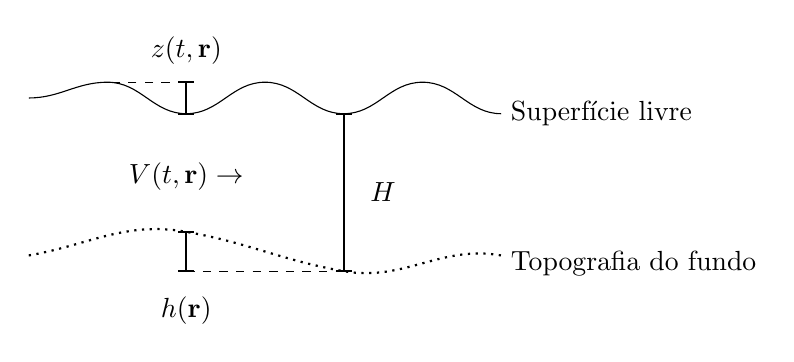
\begin{tikzpicture}[scale=1] 
						
		% Superfície livre
		\draw[above] (0,4) to[out=0,in=180] (1,4.2) 
		to[out=0,in=180] (2,3.8)
		to[out=0,in=180] (3,4.2)
		to[out=0,in=180] (4,3.8)
		to[out=0,in=180] (5,4.2)
		to[out=0,in=180] (6,3.8);
		\node[right] at (6,3.8) {Superfície livre};
						
		% Linha tracejada de referência para z
		\draw[dashed] (2,4.2) -- (1,4.2);
						
		% Desvio da superfície z
		\draw[thick] (2,3.8) -- (2,4.2);
		\draw[thick] (1.9,3.8) -- (2.1,3.8); % traço inferior
		\draw[thick] (1.9,4.2) -- (2.1,4.2); % traço superior
		\node[above] at (2,4.3) {$z(t,\mathbf{r})$};
						
		% Velocidade V(t,r)
		\node at (2,3) {$ V(t,\mathbf{r}) \rightarrow$};
						
		% Profundidade média H
		\draw[thick] (4,3.8) -- (4,1.8);
		\draw[thick] (3.9,3.8) -- (4.1,3.8); % traço superior
		\draw[thick] (3.9,1.8) -- (4.1,1.8); % traço inferior
		\node at (4.5,2.8) {$H$};
						
		% Topografia do fundo (curva inferior)
		\draw[dotted, thick] (0,2) to[out=10,in=170] (2,2.3) 
		to[out=350,in=170] (4,1.8) 
		to[out=350,in=170] (6,2);
		\node[right] at (6,1.9) {Topografia do fundo};
						
		% Variação da topografia h
		\draw[thick] (2,2.3) -- (2,1.8);
		\draw[thick] (1.9,2.3) -- (2.1,2.3); % traço superior
		\draw[thick] (1.9,1.8) -- (2.1,1.8); % traço inferior
		\node[below] at (2,1.6) {$h(\mathbf{r})$};
						
		% Linha tracejada de referência para h
		\draw[dashed] (2,1.8) -- (4,1.8);
						
	\end{tikzpicture}
	\caption{Diagrama do modelo de água-rasa adaptado}
	\label{fig:fluido-topografia}
\end{figure}

Além disso, o modelo de água-rasa adaptado é expresso por:
\begin{align}
	\frac{\partial V}{\partial t} & = - ( V \cdot \nabla)V - f \mathbf{k} \times V - g \nabla z + \nu \nabla^2 V \label{eq:agua-rasa-modificada-1}     \\
	\frac{\partial z}{\partial t} & = - (V \cdot \nabla)(z - h) - (H + z - h)\nabla \cdot  V + \kappa \nabla^2 z + F \label{eq:agua-rasa-modificada-2} 
\end{align}

Onde:
\begin{itemize}
	\item $H$: profundidade média do fluido;
	\item $h(\mathbf{r})$: variação da superfície topológica;
	\item $V(t,\mathbf{r})$: Velocidade horizontal;
	\item $z(t,\mathbf{r})$: altura da superfície;
	\item $F$: forças externas;
	\item $\kappa$: coeficiente de difusão viscosa;
	\item $\nu$: coeficiente de difusão térmica;
\end{itemize}

Em seguida, aplicamos a \textit{decomposição de Helmholtz}\footnote{Definição apresentada no apêndice \ref{app:apendice-consideracoes-matematicas} } à equação \eqref{eq:agua-rasa-modificada-1}, escrevendo
\begin{equation*}
	V = \nabla \chi + \mathbf{k} \times \nabla \psi,
\end{equation*}
onde $\chi$ é o potencial de velocidade associado à parte divergente e $\psi$ a função corrente associada à parte rotacional. Dessa forma, $\nabla^2 \chi$ representa a divergência e $\nabla^2 \psi$ a vorticidade. Substituindo essa decomposição obtemos:
\begin{align}
	\frac{\partial \nabla^2 \chi}{\partial t} & = -\tfrac{1}{2}\nabla^2(\nabla \chi \cdot \nabla \chi) 
	- \nabla \chi \cdot \nabla(\nabla^2\psi) \times \mathbf{k} 
	+ \nabla^2(\nabla \chi \cdot \nabla \psi \times \mathbf{k}) \nonumber \\
	                                          & \quad + \nabla \cdot (\nabla^2\psi\nabla\psi)          
	- \tfrac{1}{2}\nabla^2(\nabla \psi \cdot \nabla \psi) 
	+ \nu\nabla^4\chi + f\nabla^2\psi - g\nabla^2z, \label{eq:equacao-basica-1} \\
	\frac{\partial \nabla^2 \psi}{\partial t} & = -\nabla \cdot (\nabla^2\psi\nabla \chi)              
	- \nabla \psi \cdot \nabla(\nabla^2\psi) \times \mathbf{k} 
	- f\nabla^2\chi + \nu\nabla^4\psi. \label{eq:equacao-basica-2}
\end{align}

Analogamente, aplicando \eqref{eq:agua-rasa-modificada-2}, temos:
\begin{equation}
	\frac{\partial z}{\partial t} 
	= -\nabla \cdot \big[(z - h)\nabla \chi\big] 
	- \nabla \psi \cdot \nabla(z - h) \times \mathbf{k} 
	- H\nabla^2\chi + \kappa\nabla^2z + F. 
	\label{eq:equacao-basica-3}
\end{equation}

Nosso objetivo é reduzir as equações \eqref{eq:equacao-basica-1}–\eqref{eq:equacao-basica-3} a um modelo de baixa ordem. Para isso, introduzimos três vetores adimensionais $\alpha_1, \alpha_2, \alpha_3$ que satisfazem
\begin{equation*}
	\alpha_1 + \alpha_2 + \alpha_3 = 0,
\end{equation*}
e adotamos as permutações cíclicas
\begin{equation*}
	(i,j,k) = (1,2,3),\; (2,3,1),\; (3,1,2).
\end{equation*}
Definimos então:
\begin{equation*}
	a_i = \alpha_i \cdot \alpha_i, 
	\quad b_i = \alpha_j \cdot \alpha_k, 
	\quad c = (b_1b_2+b_2b_3+b_3b_1)^{1/2}.
\end{equation*}

Lorenz também apresenta uma forma alternativa, equivalente, mais conveniente para a implementação computacional:
\begin{equation*}
	b_i = \tfrac{1}{2}(a_i - a_j - a_k), 
	\quad c_i = c.
\end{equation*}

Escolhido um comprimento característico $L$, construímos três funções ortogonais:
\begin{equation*}
	\phi_i(\mathbf{r}) = \cos\!\left(\alpha_i \cdot \frac{\mathbf{r}}{L}\right),
\end{equation*}
para as quais valem, por exemplo:
\begin{align*}
	L^2\nabla^2\phi_i                              & = -a_i\phi_i,                         \\
	L^2\nabla\phi_i \cdot \nabla\phi_k             & = -\tfrac{1}{2}b_{ik}\phi_i + \cdots, \\
	L^2\nabla \cdot (\phi_j\nabla\phi_k)           & = \tfrac{1}{2}b_{jk}\phi_i + \cdots,  \\
	L^2\phi_j \cdot \nabla\phi_k \times \mathbf{k} & = -\tfrac{1}{2}c_{jk}\phi_i + \cdots, 
\end{align*}
onde os termos omitidos são múltiplos de cossenos. Com essas funções, expandimos as variáveis em série e introduzimos escalas adimensionais:
\begin{equation}\label{eq:ch01-adimensionalizacao}
    \begin{aligned}
    	t    & = f^{-1}\tau,                     \\
    	\chi & = 2L^2f^2 \sum_i x_i\phi_i,       \\
    	\psi & = 2L^2f^2 \sum_i y_i\phi_i,       \\
    	z    & = 2L^2f^2g^{-1} \sum_i z_i\phi_i, \\
    	h    & = 2L^2f^2g^{-1} \sum_i h_i\phi_i, \\
    	F    & = 2L^2f^2g^{-1} \sum_i F_i\phi_i. 
    \end{aligned}
\end{equation}

Substituindo as equações de \eqref{eq:ch01-adimensionalizacao} em \eqref{eq:equacao-basica-1}–\eqref{eq:equacao-basica-3}, e projetando sobre a base $\{\phi_i\}$, obtemos finalmente o modelo PE de baixa ordem, composto de nove equações diferenciais ordinárias:
\begin{align}
	a_i\frac{dx_i}{d\tau} & = a_ib_ix_ix_k - c(a_i - a_k)x_iy_k      
	+ c(a_i - a_j)y_ix_k -2c^2y_iy_k - \nu_0a_i^2x_i + a_iy_i - a_iz_i, \label{eq:modelo-pe-1}\\
	a_i\frac{dy_i}{d\tau} & = -a_ib_kx_iy_k - a_ib_iy_ix_k           
	+ c(a_k - a_i)y_iy_k - a_ix_i - \nu_0a_i^2y_i, \label{eq:modelo-pe-2}\\
	\frac{dz_i}{d\tau}    & = -b_kx_i(z_k - h_k) - b_i(z_i - h_i)x_k 
	+ c\,y_i(z_k - h_k) - c(z_i - h_i)y_k + g_0a_ix_i - \kappa_0a_iz_i + F_i. \label{eq:modelo-pe-3}
\end{align}

As variáveis $x_i$ representam os modos divergentes do escoamento, associados às ondas de gravidade; as variáveis $y_i$ correspondem aos modos rotacionais (vorticidade), ligados às oscilações quasi-geostróficas; e as variáveis $z_i$ funcionam como variáveis auxiliares acopladas ao sistema.

Na construção do modelo QG, começamos desprezando todos os termos não lineares, assim como aqueles que envolvem as variáveis $x$, incluindo a derivada temporal, na equação \eqref{eq:modelo-pe-1}. Fazemos o mesmo com os termos não lineares ou topográficos que dependem de $x$ nas equações \eqref{eq:modelo-pe-2} e \eqref{eq:modelo-pe-3}. Por fim, eliminamos as variáveis $x$ e $z$, obtendo ao modelo QG apresentado a seguir:
\begin{equation}
	(a_i g_0 + 1)\,\frac{dy_i}{d\tau} 
	= g_0 c (a_k - a_j) y_j y_k 
	- a_i (a_i g_0 \nu_0 + \kappa_0) y_i 
	- c h_k y_j + c h_j y_k + F_i,
	\label{eq:modelo_lorenz_deterministico_qg}
\end{equation}

\textbf{ADICIONAR SOBRE O CAPÍTULO 2.7 DO SALMON}

\section{Simulações} \label{sec:ch01_simulacoes_deterministico}
Nesta seção, apresentaremos o resultados das simulações computacionais do modelo PE, expresso pelas equações \eqref{eq:modelo-pe-1}-\eqref{eq:modelo-pe-3}. Os gráficos foram gerados a partir de simulações computacionais realizadas em Julia, principalmente, com o auxílio da biblioteca \textit{SciML: Differentiable Modeling and Simulation Combined with Machine Learning} \citep{Rackauckas2017}. 

Os parâmetros usados para a simulação foram os mesmos utilizados em \citet{Lorenz1980} e \cite{Chekroun2021}. Os parâmetros estão definidos a seguir: $g_0 = \SI{8}{\meter\per\square\second}$, $a = (1, 1, 3)$, $F = (0.1, 0, 0)$ e $c = \sqrt{\tfrac{3}{4}}$, $h=(-1, 0, 0)$ e $\nu_0 = \kappa_0 = \frac{1}{48}$. As simulações foram realizadas a partir do código disponível no apêndice \ref{app:apendice-lista-de-programas}.  

\begin{figure}[H]
	\centering
	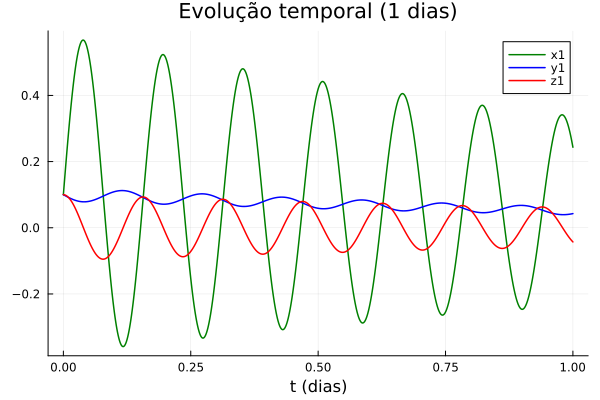
\includegraphics[width=0.6\textwidth]{00_TCC/01_LATEX/figuras/ch01_lorenz_80/evolucao_temporal_01.png}
	\caption{Simulação do modelo PE (1 dia).\label{fig:lorenz80_pe_1}}
\end{figure}



%%%%%%%%%%%%%%%%%%%%%%%%%%%% APÊNDICES E ANEXOS %%%%%%%%%%%%%%%%%%%%%%%%%%%%%%%%

% Um apêndice é algum conteúdo adicional de sua autoria que faz parte e
% colabora com a ideia geral do texto mas que, por alguma razão, não precisa
% fazer parte da sequência do discurso; por exemplo, a demonstração de um
% teorema intermediário, as perguntas usadas em uma pesquisa qualitativa etc.
%
% Um anexo é um documento que não faz parte da tese (em geral, nem é de sua
% autoria) mas é relevante para o conteúdo; por exemplo, a especificação do
% padrão técnico ou a legislação que o trabalho discute, um artigo de jornal
% apresentando a percepção do público sobre o tema da tese etc.
%
% Os comandos appendix e annex reiniciam a numeração de capítulos e passam
% a numerá-los com letras. "annex" não faz parte de nenhuma classe padrão,
% foi criado para este modelo. Se o trabalho não tiver apêndices ou anexos,
% remova estas linhas.
%
% Diferentemente de \mainmatter, \backmatter etc., \appendix e \annex não
% forçam o início de uma nova página. Em geral isso não é importante, pois
% o comando seguinte costuma ser "\chapter", mas pode causar problemas com
% a formatação dos cabeçalhos. Assim, vamos forçar uma nova página antes
% de cada um deles.

%%%% Apêndices %%%%

\cleardoublepage

\pagestyle{appendix}

\appendix
\chapter{Programas}  \label{app:apendice-lista-de-programas}

\definecolor{codebg}{RGB}{247,248,250}
\definecolor{codenumber}{HTML}{7F8C8D}
\definecolor{codekw}{HTML}{005CC5}
\definecolor{codestr}{HTML}{032F62}
\definecolor{codecm}{HTML}{6A737D}
\definecolor{codetype}{HTML}{D73A49}
\definecolor{codemacro}{HTML}{8A2BE2}

% Julia para listings
\lstdefinelanguage{Julia}{
  alsoletter={@},
  morekeywords={
    abstract,break,catch,const,continue,do,else,elseif,end,export,false,finally,
    for,function,global,if,import,let,local,macro,module,mutable,primitive,
    quote,return,struct,true,try,using,where,while,begin
  },
  morekeywords=[2]{Int,Int8,Int16,Int32,Int64,UInt,UInt8,UInt16,UInt32,UInt64,
    Float16,Float32,Float64,Complex,ComplexF64,Bool,Char,String,Nothing,Any,
    Vector,Matrix,Dict,Tuple,Union,SubArray,AbstractArray,Range},
  morekeywords=[3]{@time,@views,@inbounds,@simd,@threads,@btime,@benchmark,
    @show,@assert,@inline,@code_warntype,@test},
  sensitive=true,
  morecomment=[l]\#,
  morestring=[b]",
}

% Estilo base
\lstdefinestyle{jlstyle}{
  language=Julia,
  backgroundcolor=\color{codebg},
  basicstyle=\ttfamily\small,
  numbers=left,
  numberstyle=\scriptsize\color{codenumber},
  numbersep=8pt,
  showstringspaces=false,
  tabsize=2,
  columns=fullflexible,
  keepspaces=true,
  breaklines=true,
  frame=single,
  rulecolor=\color{codebg},
  keywordstyle=\bfseries\color{codekw},
  keywordstyle=[2]\color{codetype},
  keywordstyle=[3]\color{codemacro},
  commentstyle=\itshape\color{codecm},
  stringstyle=\color{codestr},
  upquote=true,
  % Alguns símbolos/Unicode comuns em Julia
  literate=
    {→}{{$\to$}}1 {←}{{$\leftarrow$}}1
    {≤}{{$\le$}}1 {≥}{{$\ge$}}1
    {α}{{$\alpha$}}1 {β}{{$\beta$}}1 {γ}{{$\gamma$}}1
    {π}{{$\pi$}}1 {√}{{$\sqrt{\phantom{x}}$}}1
}

% Ambiente e macro inline
\lstnewenvironment{juliacode}[1][]%
  {\lstset{style=jlstyle,#1}}{}

\newcommand{\jinline}[1]{\lstinline[style=jlstyle]!#1!}

\section{Código do modelo Lorenz 80 determinístico}
\begin{juliacode}[caption={Simulação do modelo Lorenz 80}]
using DifferentialEquations, ModelingToolkit, CSV, DataFrames

@parameters t
@variables x[1:3](t) y[1:3](t) z[1:3](t)
D = Differential(t)

a = [1.0, 1.0, 3.0]
b = [0.5 * (a[1] - a[2] - a[3]), 0.5 * (a[2] - a[3] - a[1]), 0.5 * (a[3] - a[1] - a[2])]
c = sqrt(3/4)
h = [-1.0, 0.0, 0.0]
f = [0.1, 0.0, 0.0]
g_0, kappa_0, nu_0 = 8.0, 1/48, 1/48

eqs = [
    D(x[i]) ~ (
        a[i]*b[i]*x[(i % 3) + 1]*x[((i+1) % 3) + 1]
        - c*(a[i]-a[((i+1) % 3) + 1])*x[(i % 3) + 1]*y[((i+1) % 3) + 1]
        - 2*c^2*y[i]*y[((i+1) % 3) + 1]
        - nu_0*a[i]^2*x[i]
        + a[i]*y[i] - a[i]*z[i]
    ) / a[i] for i in 1:3
]
append!(eqs, [
    D(y[i]) ~ (
        -a[((i+1) % 3) + 1]*b[((i+1) % 3) + 1]*x[(i % 3) + 1]*y[((i+1) % 3) + 1]
        - a[(i % 3) + 1]*b[(i % 3) + 1]*y[(i % 3) + 1]*x[((i+1) % 3) + 1]
        - a[i]*x[i] - nu_0*a[i]^2*y[i]
    ) / a[i] for i in 1:3
])
append!(eqs, [
    D(z[i]) ~ (
        -b[((i+1) % 3) + 1]*x[(i % 3) + 1]*(z[((i+1) % 3) + 1]-h[((i+1) % 3) + 1])
        - b[(i % 3) + 1]*(z[(i % 3) + 1]-h[(i % 3) + 1])*x[((i+1) % 3) + 1]
        + c*y[(i % 3) + 1]*(z[((i+1) % 3) + 1]-h[((i+1) % 3) + 1])
        - c*(z[(i % 3) + 1]-h[(i % 3) + 1])*y[((i+1) % 3) + 1]
        + g_0*a[i]*x[i] - kappa_0*a[i]*z[i] + f[i]
    ) for i in 1:3
])

@mtkbuild sys = ODESystem(eqs, t)

x0, y0, z0 = [0.1, 0.0, 0.0], [0.1, 0.0, 0.0], [0.1, 0.0, 0.0]
u0 = vcat(x0, y0, z0)
tspan = (0.0, 8*10.0) # 8*numero_de_dias

sol = solve(ODEProblem(sys, u0, tspan), Tsit5(); abstol=1e-6, reltol=1e-8, saveat=0.01)

U = Array(sol)
df = DataFrame(time = sol.t, x1 = U[1,:], x2 = U[2,:], x3 = U[3,:], y1 = U[4,:], y2 = U[5,:], y3 = U[6,:],z1 = U[7,:], z2 = U[8,:], z3 = U[9,:])

cd(@__DIR__)  
isdir("data") || mkdir("data")
CSV.write("data/solucao.csv", df)
\end{juliacode}

%\addappheadtotoc acrescenta a palavra "Apêndice" ao sumário; se
% só há apêndices, sem anexos, provavelmente não é necessário.
\addappheadtotoc

%%!TeX root=../tese.tex
%("dica" para o editor de texto: este arquivo é parte de um documento maior)
% para saber mais: https://tex.stackexchange.com/q/78101

\chapter{Glossário de geofísica}\label{cap:apendice_01_glossario}

\begin{itemize}
    \item \textbf{Quasi-geostrófico.}
    \item \textbf{Parâmetro de Coriolis.}
    \item \textbf{Equilíbrio hidrostático.}
\end{itemize}

\par

%%%% Anexos %%%%

\cleardoublepage

\pagestyle{appendix} % repete o anterior, caso você não use apêndices

\annex

% \addappheadtotoc acrescenta a palavra "Anexo" ao sumário; se
% só há anexos, sem apêndices, provavelmente não é necessário.
\addappheadtotoc

\par


%%%%%%%%%%%%%%% SEÇÕES FINAIS (BIBLIOGRAFIA E ÍNDICE REMISSIVO) %%%%%%%%%%%%%%%%

% O comando backmatter desabilita a numeração de capítulos.
\backmatter

\pagestyle{backmatter}

% Espaço adicional no sumário antes das referências / índice remissivo
\addtocontents{toc}{\vspace{2\baselineskip plus .5\baselineskip minus .5\baselineskip}}

% A bibliografia é obrigatória

\printbibliography[
  title=\refname\label{sec:bib}, % "Referências", recomendado pela ABNT
  %title=\bibname\label{sec:bib}, % "Bibliografia"
  heading=bibintoc, % Inclui a bibliografia no sumário
]

\printindex % imprime o índice remissivo no documento (opcional)

\end{document}
